\documentclass{elsarticle}
\usepackage{amssymb}
\usepackage{graphicx}
\journal{Decision Support Systems}
\begin{document}

\begin{frontmatter}


\title{An Integrated Decision Support System for 
Reviewer Assignment of R\&D Projects}
%\tnotetext[t1]{This document is a collaborative effort.}
%\tnotetext[t2]{The second title footnote.}

% use optional labels to link authors explicitly to addresses:
% \author[label1,label2]{}
% \address[label1]{}
% \address[label2]{}

\author[buaa]{Jun Wang\corref{cor1}}
\ead{king.wang@buaa.edu.cn}
\author[buaa]{Yunpeng Wu\corref{cor2}}
\ead{yunpeng.wu@sem.buaa.edu.cn}
\author[hk]{Jian Ma\corref{cor2}}
\ead{xx@gmail.com}
\author[hk]{Yong-hong Sun\corref{cor2}}
\ead{xx@gmail.com}


\cortext[cor1]{Corresponding author}
\cortext[cor2]{Principal corresponding author}
\fntext[fn1]{This is the specimen author footnote.}
\fntext[fn2]{Another author footnote, but a little more longer.}



\address[buaa]{School of Economics \& Management, Beihang University, Beijing 100083,
P.R. China }
\address[hk]{Department of Information Systems, City University of Hong Kong Kowloon, Hong Kong}


\begin{abstract}
% Text of abstract
In R\&D projects selection, assigning the most appropriate
experts to the relevant proposals fleetly is a very significant issue . This research aims at
developing an integrated decision support system for the reviewer assignment of R\&D projects. In this system, both knowledge of assignment experts and operations research techniques are used to
model the reviewer assignment of R\&D projects. Besides, an Assignment decision support system (ADSS) based on multi-criteria decision model
with knowledge rules is implemented. An application of a real government funding agencies in China is followed. Computational results of both effectiveness and efficiency are also provided. 
\end{abstract}

\begin{keyword}
% keywords here, in the form: keyword \sep keyword

% PACS codes here, in the form: \PACS code \sep code

% MSC codes here, in the form: \MSC code \sep code
% or \MSC[2008] code \sep code (2000 is the default)
Knowledge Acquisition; Domain Text; Theme Logic Model; Artificial Neural Network; Failure Analysis Report


\end{keyword}

\end{frontmatter}

\section{Introduction}
\label{sec:introduction}
The selection of research and development (R\&D) projects is an
important task to government funding agencies, universitie and 
research institutions, which often includes multiple
stages. Generally  the initial stage is the call for proposals (CFP), distributed to the relevant communities, such as universities and research institutions.
Proposals are submitted to the body (e.g., funding agencies) issuing
the CFP and then sent to experts for the peer review. Experts normally
review the proposals according to the instructions on the rules and
criteria of the funding agency. The review results are collected and
ranked based on the aggregation methods. For example, there are six
stages for the R\&D project selection in the National Natural Science
Foundation of China (NSFC), including Proposal submission, Assignment
of external reviewers, Peer review, Aggregation of review results,
Panel evaluation, and Final decision [1, 17]. Figure 1 shows the
process of the R\&D project selection. Because the funding decision
relies greatly on peer review results, assigning suitable referees
to review R\&D project proposals is an important research issue within
these stages.
\begin{figure}
  \centering
   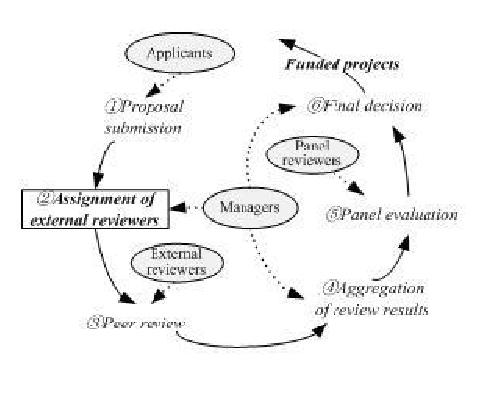
\includegraphics{figures/1.eps}
  \caption{The process of the R\&D projects selection}

\end{figure}


However, reviewer assignment in R\&D project selection has received
seldom attention. According to our literature review, only Cook et
al. [2] made efforts on this research issue. In his study, peer review
is based on partial ordinal rankings of proposals, so the objective
function of reviewer assignments is to maximize overlapping among the
subsets of proposals assigned to the various reviewers. Then the
effective final overall ranking can be obtained. It is debateable, though, since it is difficult for reviewers to select R\&D projects by pair-wire ranking if the amount of proposals is large. %Obviously, more efforts are needed in this research issue.


Similary research can be also found in the field of Operational
Research and Decision Support System. In fact, assignment problem is a
very traditional problem in Operational Research, and has been
studying in the past 50 years or so. A lot of methods are developed to
solve this kind of problems. For the standard assignment problem, the
Hungarian method proposed by H.W. Kuhn [3] can be used to obtain the
optimal solution(s). For other types of assignment problems with more
complex formats, they can be considered as the special cases of 0-1
integer programming or transportation problem. Methods such as Branch
and Bound method [4, 5, 6], cutting plane technologies [7, 8] and
their numerous improvements can be used to help to find optimal
solutions. Most of these methods, nevertheless, require rigorous
assumptions and only can solve well-structured problems [9] which may
seem not apropriate to reviewer assignment issue. Reviewer assignment
in R\&D project selection usually deals with not only well-structured
problems, but also semi-structured or ill-structured problems:
\begin{enumerate}
\item  avoiding conflicts of interests between reviewers and
  applicants is a key problem in the assignment process,
\item  on the other hand, improving the validity and efficiency of reviewer assignment is also a key problem, but these problems can’t be solved well unless we combine the knowledge of the decision maker with the decision model through establishing the ADSS.
  
\end{enumerate}

During the past few years, a number of decision models and methods
(e.g. Mathematical Programming and Optimization, Decision Analysis,
Economic Models, and Interactive Method) have been developing to help
managers make better decisions in R\&D project selection [10,
11]. However, current research findings [12, 13] indicate that many of
the elaborated decision models and methods are not being used, and
they have limited impacts on decision makings for de-facto project
selection. In order to improve the usability of decision models and
methods in real application, decision support systems (DSSs) have been
proposed and developed, which integrate decision models and methods
with computer-based supports together [1,12,14,15,16,17]. Although
some of the proposed DSSs are useful, they use decision models and
methods for specific tasks and fail to integrate the operations
research techniques into expert system. Since the R\&D project
selection process typically involves a large number of reviewers and
applicants, and there are many conflicts of interest between them
which should be taken into consideration. 

The objective of this paper is to present an integrated decision
support system to assist the reviewer assignment of R\&D projects. We
use operation research models to handle well-structured decision
problems and appropriate knowledge rules for ill-structured decision
situations. They complement each other and provide powerful supports
to the assignment processes. The proposed system is applied to the
assignment process of Natural Science Foundation of China (NSFC). Meanwhile, it can be easily modified to apply to other situations.

This paper organizaed as follows. Section 2 describes the research
background. Section 3 proposes the process of reviewer assignments of
R\&D projects and an approach which integrates knowledge of experts
and operations research model, to assign peer reviewers to proposals
for project selection. Section 4 proposes the architecture of ADSS and
the implementation of it. Section 5 discussed the application of the proposed approach in a real government funding agencies. A summary of the contribution and limitations can be found in the last section.

\section{Background}
\label{sec:background}

Founded in 1986, the NSFC is the largest government funding agencies
in China with the primary aim to promote basic and applied research
[32]. There are seven scientific departments responsible for the
selection and management of research projects. According to the
scientific research areas, they are classified into mathematical and
physical sciences, chemical sciences, life sciences, earth sciences,
engineering and material sciences, information sciences, and
management sciences. Departments are further divided into 38 divisions
with different focus on more specific research areas. For example, the
department of Management Science is further divided into three
divisions, such as Management Science \& Engineering, Macro Management
\& Policy and Business Administration. Furthermore, divisions are
further divided into different discipline areas. NSFC maintains a
dictionary of discipline areas that forms a tree structure as Figure 2 shows. The closer a discipline node is to the root, the larger discipline area it represents. For example, keyword ‘A01’ stands for ‘Mathematics’, and ‘A0101’ stands for ‘Foundation Mathematics’, and ‘A010103’ stands for ‘Geometry’ and ‘A01010302’ for ‘Algebraic Geometry’. Every year, NSFC receives a great number of project proposals (e.g., over 63,000 proposals in 2006). The project selection process is coordinated by the top management and accomplished by the seven scientific departments as well as their divisions [1]. The overall project selection task is decomposed and assigned to departments, and departments further decompose their tasks and assign to divisions. Division managers then assign external reviewers to evaluate proposals. It maintains an external reviewer database with more than 60,000 records [1, 17].






\end{document}
